\chapter{Sistema MultiAgente.}\label{cap:capitulo6}
En este capítulo se va a presentar la solución que se ha escogido para llevar a cabo la conciliación de conceptos completa de todo el sistema de etiquetado: un Sistema MultiAgente (SMA).

En este SMA van a convivir un conjunto de agentes encargados de realizar la conciliación por pares de usuarios, como se ha visto en el Algoritmo de Conciliación presentado en el capítulo~\ref{cap:capitulo4}, de forma que al final la ejecución de este SMA, el resultado sea el conocimiento conciliado para todos los usuarios que forman parte del Sistema de Etiquetado.





\section{Introducción a JADE.}

En el capítulo anterior se ha explicado que el Conjunto de Datos de Pruebas está formado por un conjunto de Usuarios, un conjunto de Objetos (Enlaces), un conjunto de Atributos (Etiquetas), y un conjunto de Tuplas \emph{usuario-objeto-atributo}.

Este Conjunto de Datos representa precisamente un Sistema de Etiquetado. Recordemos que en el  caso de este trabajo, como se comentó en el capítulo anterior, se ha seleccionado como conjunto de datos de prueba, un subconjunto de datos de Delicious (\cite{delicious}).

Por otra parte, se dispone de un Algoritmo de Conciliación (descrito en \cite{algoritmo}) que, dado un par de usuarios, calculará el conocimiento conciliado a partir de un Lenguaje Común (o conjunto de atributos comunes) y los Contextos Reducidos (o conjunto de objetos que poseen uno o más atributos de este Lenguaje Común) de cada usuario.

Por tanto, el primer problema es elegir un criterio para seleccionar los pares de usuarios que van a realizar entre ellos un proceso de conciliación. En nuestro caso, el criterio elegido es {\bf el número de objetos (enlaces) comunes} del par. Se ha elegido este criterio porque es una buena forma de obtener un Contexto Común con un número de objetos aceptable, de forma que sea más fácil sacar conclusiones. Otros criterios, como por ejemplo el número de atributos comunes (Lenguaje común), pueden ser considerados en un futuro para analizar el funcionamiento del Algoritmo y extraer otras conclusiones diferentes. En cualquier caso, en este caso, se ha usado este criterio pensando que va a ser con el que más y mejores conclusiones nos aporten los resultados.

La herramienta elegida para modelar el SMA es JADE (\cite{jade}). A continunación se detallan algunas características de este sistema. 

JADE (\emph{Java Agent Developement Framework}) es una herramienta de SMA que ofrece, principalmente, dos servicios. Por una parte, se tiene todo el entorno de computación que permite crear la plataforma dónde convivirán los agentes. Por otra, JADE ofrece todas las herramientas de programación (librerías) para crear los agentes y sus comportamientos en el sistema.

JADE es un software libre (bajo licencia LPGL) desarrollado por Tilab y está completamente realizado en Java, por lo que es posible la utilización de otros paquetes Java para ser incluidos en el código: esto permite que sea un sistema fácilmente extensible y amplio, debido a las innumerables librerías Java que existen. Además, es perfectamente portable, ya que para ser ejecutado, únicamente hace falta que el dispositivo cuente con la JVM (Java Virtual Machine), como cualquier otro programa Java.

En cuanto a la plataforma JADE, ésta se basa en una arquitectura FIPA, que establece estándares para SMA y sus agentes. Se puede consultar \cite{fipa} para más detalles (técnicos) sobre esta arquitectura. Es una plataforma distribuida, por lo que se puede ejecutar en diferentes máquinas. Esto es una característica importante, ya que al ser una plataforma distribuida, la carga de cálculo se reparte entre todas las máquinas que participen en el proceso.

La plataforma del SMA se divide en contenedores, dónde los agentes viven. Todo agente debe vivir en un contenedor, aunque puede haber contenedores dónde no viva ningún agente. Por defecto, la plataforma se inicia con un contenedor genérico principal: \emph{Main Container}. Este contenedor se comporta como un contenedor más, con la única diferencia de que siempre contiene a dos agentes característicos: el AMS (\emph{Agent Management System}) y el DF (\emph{Directory Facilitory}). El agente AMS es un agente que ofrece el servicio de páginas blancas; es decir, registra a todos los agentes del sistema mientras estén vivos. El agente DF ofrece los servicios de páginas amarillas; o lo que es lo mismo, un servicio para encontrar agentes en función de los servicios que éstos ofrecen. Mientras que los registros del AMS son transparentes para el usuario (y por tanto, son fiables); los registros del DF deben ser realizados explícitamente por el usuario (y por tanto, requieren de una comprobación posterior).

La comunicación entre agentes se realiza mediante protocolos estándares (fijados por FIPA; ver \cite{fipa}), permitiendo una separación entre los niveles físicos y lógicos de programación. De esta forma, el emplazamiento real de un agente es transparente para el usuario, ya que el nivel de comunicación se realiza automáticamente por JADE. Por tanto, un agente se comunicará igual con otro que esté en la misma máquina, o en otra máquina de la misma red, o incluso en cualquier otra máquina a la que se pueda conectar por Internet.

En la figura~\ref{fig:arquitecturaJade}, se muestra un pequeño ejemplo de JADE, en el que existe una pequeña red local con cuatro máquinas, dónde se ejecutan distribuidamente dos plataformas JADE. Cada una de ellas, contiene un contenedor principal con los agentes AMS y DF. Además, la Plataforma 1 contiene a los agentes A1 (en el contenedor principal), A2 y A3 ( en el contenedor 1) y A4 (en el contenedor 2). La Plataforma 2 cuenta también con A5 (en el contenedor principal).

\begin{figure}[t]
\centering
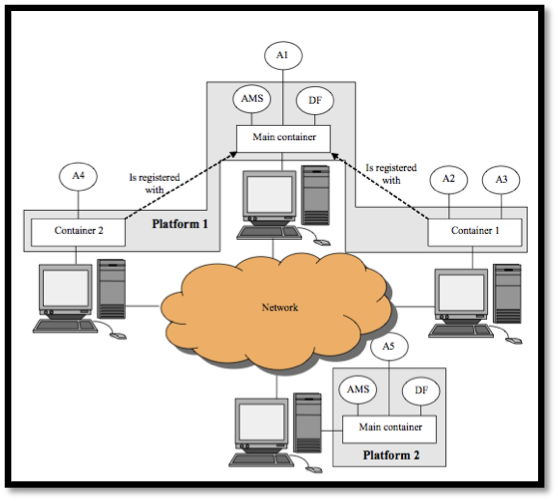
\includegraphics[scale=1]{img/6/arquitecturaJade}
\caption{Ejemplo de Arquitectura en JADE
\label{fig:arquitecturaJade}}
\end{figure}


En cuanto a las librerías que ofrece JADE, hablaremos principalmente de dos elementos: los {\bf agentes} y sus {\bf comportamientos}. Finalmente veremos las características más importantes de la {\bf comunicación}, que es el mecanismo de los agentes para interactuar.

\subsubsection{Agentes.}

Los agentes son cuerpos de ejecución, con unas funciones concretas dentro del sistema, y con capacidad de comunicación con el resto de agentes de la plataforma. En JADE, los agentes no son más que instancias de \emph{jade.core.Agent}.

Cada agente es un ente único dentro del sistema, por lo que tiene un identificador único que le diferencia del resto de agentes. Este identificador (\emph{jade.core.AID}) contiene la descripción única del agente, y tiene la siguiente estructura:

\begin{center}
	$<nickname>@<nombre\_de\_la\_plataforma>:<puerto>/JADE$
\end{center}

El ciclo de vida de un agente consta de tres partes fundamentales:
\begin{itemize}
\item Inicialización: se carga la configuración inicial del agente, y se le prepara para que empiece a funcionar.
\item Acciones: las acciones que un agente realiza se basan en los comportamientos de los que dispone. Cada comportamiento tiene unas tareas concretas, y se modelan independientes para permitir la reutilización de comportamientos por parte de varios agentes.
\item Muerte: significa el fin del agente, por lo que éste desaparece de la plataforma (y se eliminan todas las instancias de éste).
\end{itemize}

\subsubsection{Comportamientos.}


Un comportamiento no es más que una serie de instrucciones con un fin concreto. Ejemplos de comportamientos (muy simples) pueden ser sumar n números, imprimir un mensaje por pantalla, o enviar un mensaje a otro agente. Se pueden hacer comportamientos tan complejos como se puedan realizar en programación Java.

Cada agente dispone de una serie de comportamientos, organizados en dos colas: una cola controla los comportamientos activos, que el agente va gestionando para simular una ejecución paralela de todos ellos; y otra cola de comportamientos bloqueados, que se irán desbloqueando a medida que el agente reciba mensajes (por comunicación).

Un comportamiento genérico es una instancia de la clase \emph{jade.core.behaviours.\-Behaviour} y consta de dos partes:
\begin{itemize}
\item El método \emph{void action()}: son las instrucciones que forma el comportamiento en sí.
\item El método \emph{boolean done()}: indica si un comportamiento ha finalizado (y por tanto, deja de ser parte de la cola de comportamientos activos), o si el comportamiento debe seguir realizándose.
\end{itemize}

Además, existen comportamientos especiales, menos genéricos, como comportamientos que se realizan una sola vez (OneShotBehaviour), comportamientos cíclicos (CyclicBehaviour), periódicos (TickerBehaviour), por máquina de estados (FSMBehaviour), etc…

En la figura~\ref{fig:cicloVidaJade} se explica el ciclo de vida de un agente con sus comportamientos. Inicialmente, el agente se inicializa. Mientras el agente esté vivo, obtiene el siguiente comportamiento que tenga pendiente, y realiza su acción. Comprueba si el comportamiento ha finalizado y actualiza su cola de comportamientos, para coger otro comportamiento y repetir el proceso. Este proceso se repetirá hasta que el agente muera.

\begin{figure}[t]
\centering
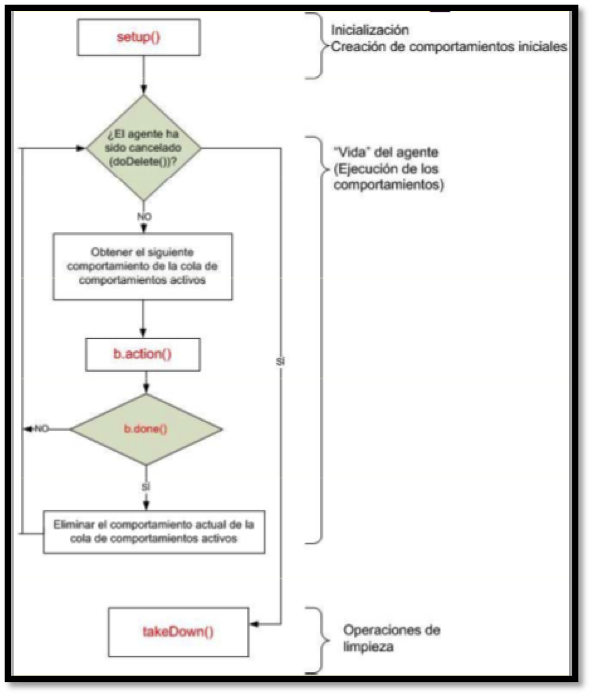
\includegraphics[scale=0.75]{img/6/cicloVidaJade}
\caption{Ciclo de vida de un agente en JADE
\label{fig:cicloVidaJade}}
\end{figure}


\subsubsection{Comunicación.}

La comunicación en JADE se realiza mediante mensajes ACL, que se basan en el estándar FIPA. Estos mensajes son instancias de \emph{jade.lang.acl.\-ACLMessage}. A grosso modo, cada mensaje consta de un receptor y un emisor, un contenido y una intención (tipo del mensaje, según la performativa con la que se mande).

La comunicación es una acción que realiza los agentes, por tanto, debe estar dentro de un comportamiento. Es común encontrar comportamientos de envío de mensajes que se producen una sola vez (OneShotBehaviour) o comportamientos de recepción continua de mensajes (CyclicBehaviour).

Normalmente, la comunicación se implementa mediante protocolos de comunicación. Existen una serie de protocolos que vienen implementados de manera estándar por FIPA. El uso de cualquier protocolo se basa en las directivas de los mensajes, de forma que, dependiendo del tipo de directiva que se reciba, se llevarán a cabo diferentes acciones. JADE implementa algunos protocolos (como FIPA Request, FIPA Query o FIPA ContractNet), y se pueden implementar otros nuevos, ya que JADE da libertad de lenguaje, soportando los lenguajes SL y LEAD (aunque se recomienda SL).

En la figura~\ref{fig:fipaRequest}, se pone el ejemplo del protocolo \emph{FIPA Request}.

\begin{figure}[t]
\centering
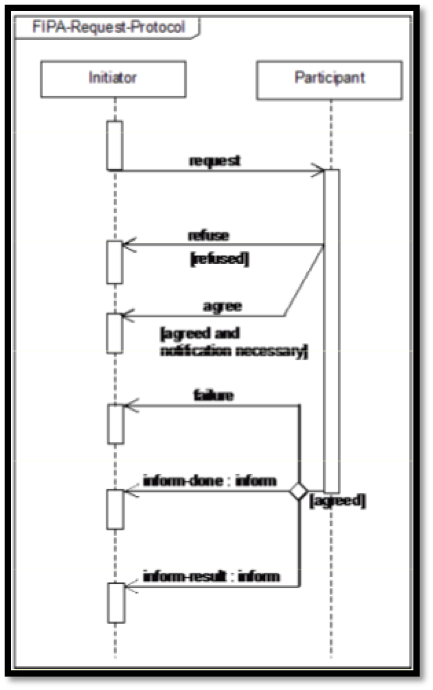
\includegraphics[scale=0.75]{img/6/fipaRequest}
\caption{Protocolo de comunicación FIPA Request
\label{fig:fipaRequest}}
\end{figure}






\subsection{Modelo de la arquitectura JADE.}

Una vez vistas las características generales de JADE en la sección anterior, se va a definir el modelo concreto de la arquitectura JADE aplicado a este trabajo; es decir, hay que definir los contenedores de nuestra plataforma de ejecución, las entidades de agentes, y sus comportamientos:

\begin{itemize}
	\item {\bf Contenedores}: Se usará el contenedor genérico (\emph{Main Container}) que JADE crea por defecto en cualquier ejecución. En este contenedor convivirán todos los agentes necesarios para la ejecución.
	\item {\bf Agentes}: Los agentes del SMA se corresponden con los {\bf Usuarios} del Conjunto de Datos de Prueba. Sin embargo, se establecerá un filtro para crear únicamente a los agentes cuya presencia sea estrictamente necesaria en la ejecución de la Conciliación. La razón para establecer este filtro es reducir el número de agentes existentes en la plataforma, ya que de no hacerse, se crearían tantos agentes como usuarios existan en nuestra base de datos; y este número es bastante alto. La consecuencia de esto sería que, muy probablemente, se diesen errores de ejecución, por desbordamiento en la plataforma debido al excesivo número de agentes en ejecución; y, por tanto, habría que buscar soluciones de implementación mucho más complejas. Sin embargo, con este filtro, se subsana este problema, y se mantiene el mismo comportamiento esperado.
	\item {\bf Comportamientos}: Dado que los agentes se corresponden con los Usuarios de un Sistema de Etiquetado, cada agente debe tener comportamientos para:
	\begin{itemize}
         	\item  Buscar otros usuarios con los que quiera conciliar su conocimiento. 
	         \item  Negociar con otros agentes si ambos están de acuerdo en comenzar una conciliación.
		\item Los comportamientos de conciliación descritos en el Algoritmo de Conciliación del capítulo 4; es decir, comportamientos para calcular el Contexto propio así como comportamientos para dialogar y negociar el conocimiento común.
	\end{itemize}
\end{itemize}







\section{Comportamiento del SMA.}

En esta sección vamos a definir el comportamiento general del SMA, describiendo cada una de las fases por las que el sistema pasa. La estructura del SMA se divide en cuatro partes: {\bf Inicialización del SMA}, {\bf Negociación entre Agentes}, {\bf Proceso de Conciliación}, y {\bf Finalización de la ejecución}.


\subsection{Inicialización del SMA.}

En la fase de Inicialización, se crearán todos los agentes que van a participar en el proceso de Conciliación. Como se ha comentado anteriormente, se va a establecer un filtro a la hora de crear a los agentes, para reducir el número de éstos en la plataforma JADE.

Primeramente, se lanzará la ejecución de la plataforma con un agente Dios (\emph{Agente Control}) cuya objetivo es buscar en el base de datos todos aquellos usuarios que superen el filtro que se elija. Por cada usuario encontrado que valide dicho filtro, se creará una nueva instancia de agente (\emph{Agente Usuario}), se introducirá en la plataforma, se le añadirán los comportamientos oportunos y se lanzará su ejecución.

El filtro que se ha seleccionado es {\bf el número de objetos (enlaces) distintos que componen el Contexto propio} de cada usuario; de forma que si este número no supera cierto umbral, dicho usuario no pasará este filtro y, por tanto, no participará en la ejecución del SMA para realizar el proceso de Conciliación con otros usuarios. Este umbral es precisamente el número de objetos (enlaces) comunes que se ha escogido para realizar la Conciliación entre dos usuarios. La justificación de este umbral es trivial: si dos usuarios concilian su conocimiento cuando poseen cierto número de objetos (enlaces) comunes, es necesario que ambos posean, al menos, ese número de objetos diferentes en su contexto propio.

Cuando un agente comienza su ejecución en la plataforma, debe inicializar las distintas variables con la información relativa al usuario que le corresponde en la base de datos. Igualmente, deberá llevar a cabo un proceso de búsqueda en la base de datos, para ver con que usuarios quiere conciliar su conocimiento. Recordemos que sólo se elegirán a aquellos usuarios que tengan un número de objetos (enlaces) comunes igual o superior a un umbral inicialmente establecido.

Al finalizar esta fase de inicialización, el resultado es una plataforma en la que están conviviendo todos los usuarios que pueden\footnote{Es posible que algunos de los agentes que conviven en la plataforma no participen en ningún proceso de Conciliación con otros usuarios; sin embargo, esto no representa ningún problema de implementación y/o ejecución.} participar en algún proceso de Conciliación con otros usuarios, y todos ellos están ejecutándose con sus comportamientos oportunos, que dependerán de cada usuario, tal y como se detalla en el siguiente apartado.





\subsection{Negociación entre Agentes.}

En esta fase, se establece un protocolo de comunicación entre los agentes, en los que se llevan a cabo paralelamente dos procesos simultáneos:

\begin{itemize}
	\item {\bf Envío de propuestas}: Cada usuario enviará propuestas para conciliar su conocimiento con otros usuarios. Estos usuarios a los que les envía propuestas, han sido calculados previamente en la fase de inicialización. Las propuestas se enviarán según la prioridad con la que quiera conciliarse con otro usuario, de forma que se comenzará enviando propuestas a aquellos usuarios que comparten muchos objetos (enlaces), y será menos prioritario para aquellos con los que comparte un número menor. Si una propuesta recibe una aceptación, ambos usuarios comenzarán el proceso de Conciliación. En caso contrario, el agente buscará otro usuario en su cola de peticiones pendientes, hasta encontrar a un usuario que acepte su petición.
	\item {\bf Recepción de solicitudes}: Cada usuario deberá implementar un procedimiento de recepción de solicitudes, de forma que pueda atender las peticiones que llegan procedentes de otros usuarios. Por norma general, todos los agentes aceptarán las peticiones entrantes que reciban, siempre y cuando no estén ejecutando un proceso de conciliación con otro agente, en cuyo caso no se procesaría dicha solicitud entrante, y por tanto se descartaría.
\end{itemize}

Hay que indicar que un usuario puede iniciar la conciliación de su conocimiento por cualquiera de los dos procesos. Sin embargo, un usuario no puede realizar varias conciliaciones de forma simultánea. Por tanto, si un usuario va a comenzar a conciliar su conocimiento con otro, se deben bloquear los dos procesos anteriores, ya que el usuario no volverá a enviar más peticiones hasta que finalice el proceso de conciliación, e igualmente no podrá atender solicitudes entrantes por la misma razón.

Puede darse el caso de que alguno de los dos procesos descritos anteriormente, bloquee la negociación del otro proceso. Es decir, ambos procesos pueden coexistir y ejecutarse sin problemas. La explicación se da por el paralelismo que ofrece JADE en cuanto a los comportamientos de los agentes; de forma que un comportamiento puede estar bloqueado (esperando que se desbloquee al recibir un mensaje), y al mismo tiempo el agente tener en ejecución otro comportamiento diferente. Por tanto, puede que un agente esté negociando al mismo tiempo con otro tras haberle enviado una propuesta (actuando como iniciador de la negociación), y a la vez con un tercero tras haber recibido una solicitud de éste último (actuando como receptor en la negociación). Se seguirá una estrategia FIFO para solucionar este problema; o lo que es lo mismo, se despachará la negociación que antes se complete, ya sea por el proceso de envío de propuestas o por el proceso de recepción de solicitudes. El otro proceso se bloqueará, y se evitará, de esta forma, que se produzcan dos conciliaciones simultáneas.

En la figura~\ref{fig:transicion}, se adjunta el diagrama de transición de estados de los agentes usuario durante su fase de Negociación y Conciliación, con las fases iniciales y finales de Inicialización y Terminación. Tras la Inicialización, se desarrollan dos comportamientos paralelos de Negociación: el envío de propuestas y la recepción de solicitudes. En este diagrama, se ve gráficamente que es imposible que un agente realice varias conciliaciones simultaneas; ya que se comprueba antes de comenzar cualquier conciliación el valor de {\tt libre}, y en caso de no estarlo, se aborta el proceso.

\begin{figure}[t]
\centering
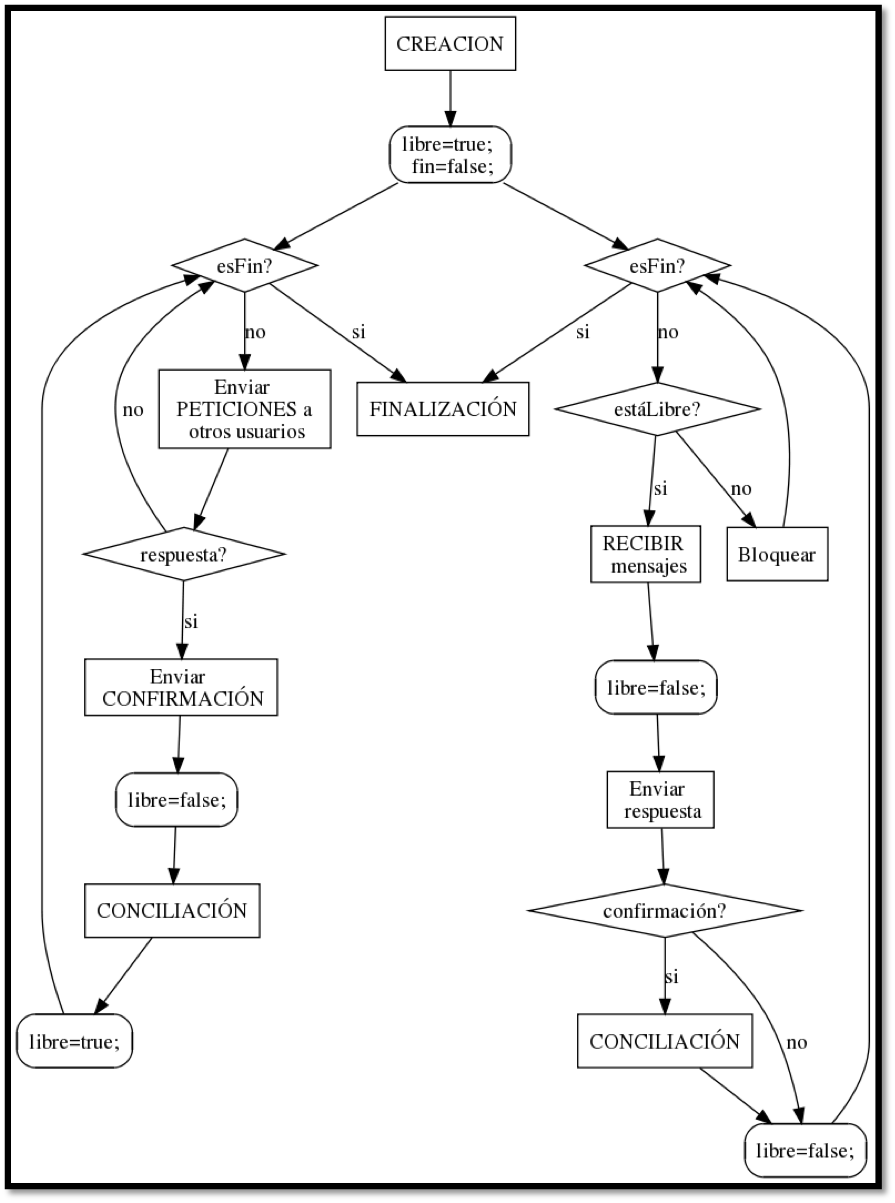
\includegraphics[scale=0.35]{img/6/transicion}
\caption{Diagrama de transición de estados de los Agentes Usuario
\label{fig:transicion}}
\end{figure}


\subsection{Proceso de Conciliación.}

El proceso de Conciliación se llevará a cabo siguiendo el algoritmo descrito en \cite{algoritmo}, que se ha explicado en el Capítulo~\ref{cap:capitulo4}. Por tanto, una vez que dos usuarios han aceptado una negociación, éstos comenzarán esta tarea mediante la cual van a conciliar su conocimiento.

Cuando un agente esté realizando la conciliación con cualquier otro agente, debe bloquear todos sus comportamientos, excepto aquellos que llevan a cabo la conciliación. De esta forma, se evitará que un agente intente negociar conciliaciones simultáneas, restrigiendo este proceso para que únicamente se realice una única conciliación con otro usuario, y que además sea el único proceso que ambos usuarios estén realizando, desde que comience la conciliación hasta que finalice.

En el capítulo~\ref{cap:capitulo4}, se describía las distintas fases del algoritmo. De estas seis fases que constituyen el algoritmo completo, se distinguen dos conjuntos de operaciones, que vamos a separar en el nivel de implementación:

\begin{itemize}
	\item {\bf Cálculos del propio usuario} (Pasos 1-2): En estos pasos se lleva a cabo la inicialización de cada uno de los agentes, y ambos extraen su Contexto personal (de la base de datos), así como sus Retículos de Conceptos y sus Bases Stem. En esta fase, no se produce ningún proceso de comunicación con el otro agente.
	\item {\bf Diálogo entre usuarios} (Pasos 3-6): En esta fase comienza el proceso de diálogo, en el que primeramente se envían y se reciben los Conjuntos de Atributos propios de cada agente (paso 3). Este paso es comunicativo, y además, supone un punto de sincronización en el algoritmo, ya que no se puede avanzar hasta que no se recibe el conjunto del otro usuario. Se continúa calculando el Contexto Reducido (paso 4) y crear un Sistema de Producción a partir de éste (paso 5). En estos pasos no hay comunicación entre agentes. Finalmente, se produce un proceso de Negociación (paso 6), a través de un envío masivo de los objetos de cada usuario, y el procesamiento de cada uno de ellos.
\end{itemize}

Es interesante la distinción de las dos fases anteriores porque: 1) la primera fase es idéntica para todos los procesos de conciliación de un usuario; mientras que la segunda es exclusiva para cada cada conciliación concreta; y 2) en la primera fase no se lleva a cabo comunicación alguna, mientras que la segunda comienza y termina por un acto comunicativo\footnote{Se entiende por {\bf acto comunicativo} al envío o recepción de un mensaje.}.

Por tanto, en el nivel de la implementación, se han realizado dos comportamientos que simulen las dos fases anteriores. La primera vez que un agente realice una conciliación, se creará un comportamiento secuencial de forma que se secuencien ambas fases. Sin embargo, a partir de la segunda conciliación que un usuario realice, la primera fase no será necesario repetirla (los Contextos, Retículos y Bases Stem quedaron guardadas la primera vez que se realizó el proceso), por lo que se llevará a cabo únicamente la segunda fase (pasos 3-6 del algoritmo).

Finalmente, se ha añadido una acción final al algoritmo, que permita almacenar los datos obtenidos en una base de datos (para su posterior procesamiento, extracción de resultados estadísticos, conclusiones, etc...). En esta acción se almacenará el contexto común que se ha obtenido, junto con los datos de ambos usuarios, para saber a quien pertenece. Hay que recordar que con la herramienta ConExp (\cite{conextp}) se puede calcular fácilmente el Retículo de Conceptos y las Bases Stem a partir de este Contexto común, que es el resultado del Algoritmo de Conciliación entre ambos usuarios.



\subsection{Finalización de la ejecución.}

La ejecución global del SMA finalizará cuando todos los usuarios hayan realizado todas las tareas de conciliación que tenían previstas con otros usuarios. Estas tareas se planifican en la fase de Inicialización del SMA, y se almacenan en una cola de peticiones pendientes para cada usuario.

Una vez que un usuario vacíe su cola de peticiones pendientes, enviará un mensaje al Agente Control, y únicamente dejará activo su comportamiento de recepción de solicitudes de otros usuarios. De esta forma, el usuario seguirá activo en la plataforma para atender peticiones entrantes.

El agente Control irá gestionando la recepción de mensajes, cuando cada usuario vacíe su cola de peticiones pendientes. De esta forma, este agente sabrá en todo momento el estado en el que se encuentra cada uno de los usuarios que participan en la plataforma. Hay que recordar que este agente Control es el creador de todos los usuarios, por lo tanto, tiene conocimiento de todos ellos.

Finalmente, el agente Control llevará a cabo una tarea de finalización del sistema una vez que el estado de todos los usuarios sea \emph{terminado}; es decir, cuando haya recibido un mensaje de finalización (por tener vacía su cola de conciliaciones pendientes) de todos los usuarios del SMA.

















\section{Componentes.}

A continuación se detallan los distintos agentes, y sus diferentes comportamientos.

\subsection{Agente Control.}

Este agente es el encargado de comenzar la ejecución del SMA. Únicamente existirá una instancia de él.

En dicho agente se define el {\bf umbral}, que es el número mínimo de objetos (enlaces) comunes que deben tener dos usuarios para realizar una conciliación de su conocimiento. Este umbral es una variable de tipo {\tt entero} mayor o igual a 0. Nótese que cuando el umbral es exactamente 0, equivale a que cada usuario concilie su conocimiento con todos los usuarios con los que comparte 0 o más objetos (enlaces); es decir, con todos los demás usuarios. Por tanto, estableciendo un umbral de 0 unidades, se produciría un proceso de conciliación completo en el sistema: todos con todos. Sin embargo, en nuestro caso, este valor se interpretará de forma excepcional, realizando únicamente la conciliación con aquellos usuarios que no tienen ningún objeto común. En cualquier caso, a nivel de implementación, se ha visto que no tiene sentido realizar conciliaciones con umbrales muy pequeños, pues los resultados son muy pobres y el coste computacional para realizarlos es muy grande. En este trabajo, el umbral mínimo con el que se trabaja es 3.

Este agente también deberá guardar información acerca del estado de los usuarios, para saber cuándo han terminado todos. Para ello, se creará un {\tt vector} de tipo {\tt boolean}, con tantas posiciones como usuarios, dónde se registrará si un usuario ha terminado o no.

Inicialmente, se establecerá el valor del umbral, se inicializará el vector sobre el estado de los usuarios a {\tt false} (ninguno ha terminado), y se añadirá el comportamiento de {\bf Buscar usuarios} al Agente Control.

\subsubsection{Comportamiento Buscar Usuarios.}

Este comportamiento es de tipo puntual ($OneShotBehaviour$), y su misión es recorrer la base de datos en busca de usuarios que superen el filtro establecido (este filtro se establece en función del umbral).

Cada vez que se encuentre un usuario válido, se añadirá un comportamiento {\bf Crear Usuario} (ver siguiente apartado) al Agente Control, al que se pasarán como parámetros los datos del usuario correspondiente.

Una vez que se ha recorrido toda la base de datos, se dará por concluido este comportamiento, aunque previamente se le añadirá al agente el comportamiento de {\bf Esperar Fin de Usuarios}.

\subsubsection{Comportamiento Crear Usuario.}

Este comportamiento es de tipo puntual ($OneShotBehaviour$). El objetivo de este comportamiento es crear una nueva instancia de Agente Usuario, introducirlo en la plataforma y comenzar su ejecución.

La creación del Agente Usuario se realiza pasando como parámetros su ID, su nombre de usuario, y también, el umbral en el que se está trabajando. Con éste último, un usuario podrá localizar a aquellos usuarios con los que debe conciliarse, y descartar a aquellos con los que no deba.

Una vez que se realizan estas operaciones, el comportamiento concluye su ejecución.

Hay que indicar que el Agente Control tendrá tantos comportamientos de este tipo como usuarios tengan que ser creados. Cada uno de estos usuarios será creado de forma independiente en ejecuciones diferentes del Agente Control.

\subsubsection{Comportamiento Esperar Fin de Usuarios.}

Este comportamiento, de tipo cíclico ($CyclicBehaviour$), tiene como misión recibir los mensajes de los distintos usuarios, que informarán cuando su cola de peticiones de conciliaciones se haya vaciado. Una vez que todos los usuarios informen de esta situación, se llevará a cabo la finalización del sistema.

Dado que este comportamiento es secundario, permanecerá bloqueado largos períodos de tiempo, en comparación con el tiempo que está ejecutándose (esperando mensajes). Por tanto, se ha establecido un tiempo de 1 segundo en el cual permanece a la escucha de mensajes entrantes, y un tiempo de 60 segundos en los que el comportamiento queda bloqueado si no ha recibido ningún mensaje. Cuando el SMA esté finalizando, es probable que muchos usuarios envíen este mensaje de finalización al Agente Control; estos mensajes serán procesados uno tras otro, sin bloqueos. Sin embargo, la razón para establecer este bloqueo tan alto es no acaparar el uso de CPU en las fases intermedias de la ejecución del SMA, y no perjudicar la ejecución de los usuarios.

La recepción de mensajes se llevará a cabo aplicando un filtro, de forma que sólo sean aceptados mensajes de tipo {\tt INFORM}. Igualmente, se procesará el campo {\tt contenido} del mensaje, para decodificar el índice del usuario dentro del SMA.

\subsubsection{Comportamiento Finalizar Sistema.}

Este comportamiento, de tipo puntual ($OneShotBehaviour$), tiene como objetivo finalizar la ejecución del SMA, debido a que se han realizado todas las conciliaciones posibles para el umbral que se había establecido inicialmente.

Por simplicidad, se ha elegido imprimir un mensaje por pantalla que nos indique que esta ejecución ha finalizado.

Como se comentará en capítulos siguientes, se podría realizar una implementación más rica con la intención de incorporar este proyecto como módulo en un proyecto de mayores dimensiones. Sin embargo, en este caso no es necesario, por lo tanto se ha optado por la solución más simple.





\subsection{Agente Usuario.}

Este agente representa a un usuario del sistema. Por tanto, existen numerosas instancias de él, para que todos los usuarios que intervienen en el proceso de conciliación estén presentes en la plataforma en forma de agente.

En su inicialización, se establecerán los valores de ID y nombre de usuario, así como el valor del umbral con el que se está trabajando. También debe almacenar la lista de usuarios con los que quiere conciliarse ({\tt Lista$<$entero$>$}). Tendrá variables que almacenen su Contexto propio (co\-mún para cualquier conciliación), así como el Contexto Reducido,  el Contexto común  y el Sistema de Producción de cada una de las conciliaciones que realice. Los tres contextos son variables de tipo {\tt Contexto}, mientras que el Sistema de producción es de tipo $StemClips$\footnote{Las clases {\tt Contexto} y {\tt StemClips} son proporcionadas como utilidad en este proyecto}. También almacenará su estado, {\tt libre} y {\tt fin}, en dos variables de tipo {\tt boolean}. Finalmente, también se guardará temporalmente los datos del usuario con el que se esté conciliando (mientras dura este proceso): su ID y su AID\footnote{El AID es un identificador de agente de JADE, que es único para cada agente de la plataforma.}.

Nótese que el umbral se define una única vez en el Agente Control. Sin embargo, su valor se va heredando a todos los agentes que componen el sistema, convirtiéndose, de esta forma, en una variable $global$\footnote{Se considera variable global a efectos prácticos, ya que todo agente la posee, y tiene el mismo valor para todos. Sin embargo, no se corresponde a la definición formal de variable global.}.

Inicialmente, comenzará con el comportamiento de {\bf Exploración de la base de datos}, y a medida que avance en su ejecución, se irán modificando dinámicamente los distintos comportamientos, como se detalla a continuación.

\subsubsection{Comportamiento Explorar Base de Datos.}

Este comportamiento es de tipo puntual ($OneShotBehaviour$). El objetivo es explorar la base de datos en busca de otros usuarios que compartan un número de objetos igual o superior al umbral establecido.

Cada uno de los usuarios que superen este filtro, serán añadidos a la lista de peticiones pendientes de este agente, que será procesada más adelante por otros comportamientos. Por cuestiones de implementación, sólo se añadirán a esta cola de peticiones, usuarios cuyo ID sea superior al del propio usuario en cuestión. La razón para hacer esto es evitar duplicidades a la hora de realizar las conciliaciones entre los diferentes usuarios. De esta forma, se reduce a la mitad el número de peticiones (mensajes) que se están enviando en la plataforma; y, por tanto, se optimizan las comunicaciones y se mejora la eficiencia.

Finalmente, antes de acabar con la ejecución de este comportamiento, se realizarán la siguientes acciones:

\begin{itemize}
	\item En caso de que la lista de peticiones pendientes sea no vacía, se añadirá al agente el comportamiento de {\bf Envío de peticiones}. En caso contrario, se enviará un mensaje al Agente Control, indicando que ha finalizado (ya que su cola de peticiones está vacía).
	\item Se añade para todos los agentes el comportamiento de {\bf Recepción de solicitudes}.
\end{itemize}

\subsubsection{Comportamiento Enviar Propuestas.}

Este comportamiento es de tipo simple ($Behaviour$); es decir, actuará de forma cíclica hasta que se cumpla una condición de fin. El objetivo de este comportamiento es llevar a cabo las negociaciones con otros usuarios para conciliar mútuamente su conocimiento. Esta negociación puede llevarse con el rol de emisor (o iniciador de la negociación), o con el rol de receptor. Este comportamiento ejecutará esta negociación con el rol de emisor.

El agente dispone de una cola de usuarios a los que desea realizarles una petición de conciliación. Hay que recordar que este comportamiento estará activo únicamente cuando esta cola sea no vacía. A medida que finalizan las diferentes conciliaciones con los usuarios que tiene pendiente, éstos se van eliminando de esta cola. La condición de fin de este comportamiento es, por tanto, el momento en el que dica cola queda vacía, ya que se habrán realizado todas las conciliaciones que este usuario tenía planificadas.

La acción que se realiza en cada ciclo, mientras el comportamiento está activo, es una negociación con otros usuarios para intentar iniciar una conciliación. Esta negociación se produce de la siguiente manera:

\begin{enumerate}
	\item En caso de estar {\tt libre}\footnote{Un usuario se considera \emph{libre} cuando no está realizando ningún proceso de conciliación con ningún otro usuario}, selecciona con mayor prioridad de su cola de peticiones pendientes, y le envía una propuesta de conciliación. Esta propuesta es un mensaje de tipo {\tt PROPOSE}. En caso de estar {\tt ocupado}, se bloquea cierto tiempo.
	\item Se bloquea cierto tiempo esperando respuesta. La respuesta debe coincidir con una plantilla previamente definida, en la que coincidan el tipo de mensaje (performativa) así como el remitente, con los valores esperados. Los mensajes aceptados, provenientes del emisor concreto, deben ser de tipo {\tt ACCEPTAL\_PROPOSE}.
	\begin{enumerate}
		\item En caso de recibir respuesta, establece su estado a \emph{ocupado}\footnote{ Un usuario establece su estado a \emph{ocupado} poniendo {\tt libre = false}.} y envía un mensaje de confirmación al otro usuario. Este mensaje es de tipo {\tt INFORM}.
		\item En caso contrario, se recomienza el proceso (paso 1), con el siguiente usuario de su cola de peticiones.
	\end{enumerate}
	\item Se comienza el proceso de Conciliación con el otro usuario.
	\item Al finalizar la conciliación, se establece el estado del usuario a \emph{libre} y se elimina al usuario con el que ha conciliado su conocimiento de la cola de peticiones pendientes.
	\item Si su cola de peticiones queda vacía, se enviará un mensaje al Agente Control, indicando que ha finalizado, y se finaliza el proceso. En caso contrario, éste se reinicia.
\end{enumerate}

Es importante indicar que, además de atender mensajes que sean aceptados por la plantilla anteriormente definidas, se llevará a cabo un proceso de limpieza de la cola de mensajes del agente antes de recibir cualquier mensaje, para que no sean atendidos, incorrectamente, mensajes que llegaron en negociaciones anteriores. De esta forma, se garantiza que el protocolo de negociación es totalmente fiable y robusto, de forma que dos usuarios comenzarán el proceso de conciliación si ambos están listos para conciliarse con el otro. En ningún caso, se darán la circunstancia de que un agente comience a conciliarse con otro mientras este otro esté negociando con otros terceros agentes.

En concreto, esta cola de mensajes se vaciará antes de enviar el mensaje de propuesta ({\tt PROPOSE}), ya que previamente elimina todos los mensajes de tipo {\tt ACCEPTAL\_\-PROPOSE} cuyo remitente sea el mismo al que se le está enviando la propuesta. Hay que recordar que JADE almacena una cola de mensajes, en la que éstos quedan almacenados hasta que el agente los lea. Esta cola es de tipo \emph{FIFO (First In First Out)}. Por tanto, se puede dar el caso que en un agente receptor aceptara en el pasado una propuesta, y enviara su correspondiente mensaje de aceptación. Sin embargo, si este mensaje no llega en los umbrales de tiempo establecidos, la negociación no se aceptará; teniendo que reiniciarse esta negociación con este usuario en un futuro. Ésta es la razón por la cual pueden existir aceptaciones guardadas en la cola de mensajes del agente. Por tanto, vaciarla la cola de mensajes nos permite asegurar que el protocolo de negociación se ejecutará correctamente.

Igualmente, si algún mensaje se pierde en el proceso, no ocurrirá nada ya que el protocolo está pensado para que se reinicie en caso de no recibir la respuesta del otro agente. Al reiniciar, se comenzará la negociación otros usuarios. La pérdida de mensajes puede deberse a fallos en las comunicaciones u otros motivos externos a la plataforma JADE.





\subsubsection{Comportamiento Recibir Solicitudes.}

Este comportamiento, de tipo cíclico ($CyclicBehaviour$), tiene como objetivo recibir y atender las solicitudes de conciliación que el usuario recibe. En este comportamiento, el usuario asume el rol de receptor en la negociación.

Como norma general, un usuario aceptará siempre cualquier solicitud que reciba, excepto en el caso de que se encuentre ocupado con otra negociación. Por tanto, como regla general, un usuario gestionará primeramente las conciliaciones que le llegan como solicitud que aquellas que tiene pendiente para ser propuestas a otros usuarios. Sin embargo, esta regla está condicionada al momento en el que llegan los mensajes; por lo que es posible que cierto usuario gestione inicialmente una propuesta propia que una solicitud externa. En cualquier caso, la regla anterior se cumple en la mayoría de los casos. Hay que recordar que para cierto par de usuarios que deseen conciliar su conocimiento entre ambos, únicamente el usuario con menor ID será el que tenga al otro usuario en su cola de propuestas pendientes; de esta forma se evita duplicidad y posibles bloqueos indefinidos en la negociación mútua; asegurando que en algún momento se llevará a cabo la conciliación entre ambos.

En cada ciclo, la negociación para el proceso de recepción de solicitudes que se lleva a cabo está compuesta por las siguientes acciones:

\begin{enumerate}
	\item En caso de estar \emph{libre}, atiende los mensajes entrantes. Dichos mensajes deben coincidir con una plantilla en la que se especifica el tipo de mensajes ({\tt PROPOSE}). En caso contrario, se bloquea cierto tiempo.
	\item Cuando llega una propuesta, establece su estado a \emph{ocupado}, y envía un mensaje de aceptación (de tipo {\tt ACCEPTAL\_PROPOSE}). Volverá a bloquearse cierto tiempo esperando la confirmación del otro usuario, para comenzar la Conciliación. Esta confirmación deberá coincidir con cierta plantilla, en la que sólo se aceptan mensajes de ese remitente, y de tipo {\tt INFORM}.
	\begin{enumerate}
		\item En caso de recibir dicha confirmación, se comienza el proceso de Conciliación. Al finalizar, el agente deberá establecer su estado a \emph{libre}.
		\item En caso de no recibir respuesta, se establece el estado a \emph{libre} y se reinicia el proceso para atender nuevas peticiones.
	\end{enumerate}
\end{enumerate}

Igual que en el caso del comportamiento anterior, para que el protocolo de negociación funcione correctamente, se vaciarán las colas de mensajes entrantes. En concreto, se lleva a cabo una limpieza del buffer de mensajes después de recibir la solicitud; de forma que si un usuario realizó varias peticiones consecutivas en el pasado (peticiones que aún no habían sido procesadas), se eliminan todas ellas, para que no haya errores en el futuro debido a solicitudes no procesadas.



\subsubsection{Comportamiento Calcular Contexto Propio.}

Este comportamiento, de tipo puntual ($OneShotBehaviour$), tiene como objetivo realizar los pasos 1 y 2 del Algoritmo de Conciliación; es decir, inicializar la conciliación, construir el Contexto personal y calcular el Retículo de Conceptos relativo a este contexto así como sus Bases Stems asociadas. Además, este comportamiento sólo se realizará, como máximo, una vez por parte de cada usuario; ya que estos cálculos no varían y son muy costosos computacionalmente. Por tanto, en el momento en que el usuario vaya a llevar a cabo su primer proceso de conciliación con otro usuario, se harán los cálculos oportunos, y éstos quedarán almacenados en la memoria del propio agente, para que puedan ser usados en futuras conciliaciones.

La construcción del Contexto propio es un proceso de exploración en la base de datos, para obtener:

\begin{itemize}
	\item El Lenguaje propio: conjunto de Atributos (etiquetas) que el usuario utiliza.
	\item El conjunto de Objetos (enlaces) que el usuario ha etiquetado.
	\item Las relaciones entre ambos.
\end{itemize}

Una vez que se ha construído este contexto, se puede calcular fácilmente los Conceptos del usuario así como sus Bases Stem, mediante las llamadas opotunas a las librerías de ConExp (ver \cite{conexp}).




\subsubsection{Comportamiento Dialogar Conciliación.}

Este comportamiento es la secuencia de los pasos 3 a 6 del Algoritmo de Conciliación. Para implementarlo, se ha escogido un comportamiento simple ($Behaviour$), en el que al inicio de cada acción, se evaluará el paso que se debe realizar y se ejecutará correspondientemente; y al final de cada uno de ellos, se establecerá un nuevo valor para ejecutar el paso siguiente. La condición de fin es, evidentemente, el momento en el que finaliza el paso 6 de este algoritmo.

A continuación se detallan los diferentes estados que se han definido, y se detallan las acciones que se realizan en cada uno de ellos:
\begin{itemize}
	\item Estado = 0 (Paso 3). Se inicia el diálogo enviando el lenguaje propio del usuario; es decir, el conjunto de atributos que el usuario utiliza. 
	\item Estado = 1 (Paso 3 y 4). Se bloquea hasta recibir el lenguaje del otro usuario, que será un mensaje de las mismas características que el que él ha enviado. Con el mensaje recibido, se puede calcular el Contexto reducido propio, que será una reducción del contexto propio al lenguaje común. El lenguaje común no es más que la intersección entre el lenguaje propio y el lenguaje recibido. Este contexto reducido estará formado por el conjunto de atributos que forman parte del lenguaje común, así como todos aquellos objetos que estén etiquetados con alguno de estos atributos, eliminando de éstos todas las etiquetaciones de etiquetas que no pertenecen al lenguaje común. Una vez calculado este Contexto reducido, se pasará al estado siguiente. En caso de que dicho contexto no contenga objetos, se pasará al estado 5.
	\item Estado = 2 (Paso 5). Se sintetizará un Sistema de Producción a partir de las Bases Stem del Contexto reducido calculado anteriormente.
	\item Estado = 3 (Auxiliar). Se enviará al otro usuario el número de objetos del contexto reducido, y se bloqueará hasta recibir el mismo tipo de mensaje del otro usuario. Este paso es meramente auxiliar y no está especificado en el Algoritmo de Conciliación. Sin embargo, si ambos usuarios conocen el número de objetos totales con los que se está trabajando, se podrá establecer fácilmente una condición de fin para el paso 6.
	\item Estado = 4 (Paso 6). Inicialmente se realizará un envío masivo de todos los objetos del usuario. Posteriormente, se irán procesando todos los mensajes entrantes, hasta que se dé la condición de fin. Como se describe en el capítulo~\ref{cap:capitulo4}, el paso 6 del Algoritmo genera tres posibles respuestas a cada mensaje recibido: aceptación si se satisfacen todas las implicaciones; proposición de un nuevo objeto, si se genera alguna sugerencia después de procesarlo en el sistema de producción; o rechazo en caso contrario. La clave de este estado está en establecer la condición de fin. En el estado anterior, hemos capacitado al usuario para que conozca el número de objetos del otro usuario (por supuesto, el número de objetos propio también lo conoce). Por otra parte, un objeto habrá terminado de procesarse cuando se produzca una aceptación o un rechazo del mismo. Mientras que si el resultado es una nueva proposición, el objeto $evoluciona$ y se genera una nueva proposición. Sin embargo, se puede tener un control de los objetos iniciales que generan nuevas proposiciones. Por tanto, se fijará el campo {\tt conversationID} de los mensajes, indicando el usuario que inicia el proceso y el índice del objeto que se está procesando. De esta forma, se controla el fin del procesado de cada objeto. La condición de fin será, por tanto, cuando se hayan procesado todos los objetos, tanto los propios como los del otro usuario. Además, se añadirá la posibilidad de fin por límite de tiempo, que se dará en aquellos casos en los que algún mensaje se pierda y no sea recibido. El límite de tiempo fijado será de 60 segundos. Pasado este tiempo, se finalizará igualmente este paso.
	\item  Estado = 5 (Auxiliar). Para un procesamiento posterior, se almacenará en una base de datos, el contexto común calculado, resultado de la conciliación de ambos usuarios. Para evitar duplicidades en la base de datos, esta operación únicamente la realizará el usuario con menor ID.
	\item Estado = 6 (Fin). Se finaliza el comportamiento.
\end{itemize}

Hay que añadir que en todos los estados en los que interviene un proceso comunicativo\footnote{Se entiende proceso comunicativo aquel en el que se hay acciones de envío de mensajes o acciones de recepción.}, se establecerán límites de tiempo para que, si se supera este límite, el proceso se finalice, evitando que el agente quede bloqueado. La justificación para realizar esta implementación es la posibilidad de que ciertos mensajes se pierdan. Normalmente, cuando la plataforma JADE funciona en una única máquina (localmente), no se pierde ningún mensaje. Sin embargo, cuando la plataforma se ejecuta de forma distribuida, los procesos comunicativos de la plataforma quedan sujetos a los protocolos de comunicación de la propia máquina dónde se esté ejecutando. Por ejemplo, si una máquina perdiese la conexión con la red, todos los agentes que se ejecutan en dicha máquina se desconectarían y no continuarían su normal ejecución.


\section{Notas de Implementación y Ejecución.}

Es interesante indicar las siguientes notas sobre la implementación y la ejecución:

\begin{itemize}
	\item En el apartado de implementación, sólo se han implementado las clases relativas al SMA. El resto de clases para trabajar con Objetos, Atributos, Contextos, Sistema de Producción, etc...; han sido reutilizadas de una implementación anterior.
	\item El Algoritmo de Conciliación presentado en \cite{algoritmo} se ha implementado por completo.
	\item Además de las clases no implementadas comentadas anteriormente, la parte implementada del proyecto se encuentra dentro del paquete {\tt sma}. Dentro de éste encontramos las clases del agente Control y sus comportamientos. Además, se encuentran otros subpaquetes: {\tt sma.templates}, {\tt sma.users} y {\tt sma.util}. En el paquete {\tt sma.templates} se encuentra la implementación de algunas plantillas que se usarán para filtrar la recepción de mensajes. En el paquete {\tt sma.users} se encuentra la implementación del Agente Usuario y sus comportamientos. Finalmente, en el paquete {\tt sma.util} se encuentran algunas clases auxiliares, como por ejemplo, la que nos permite establecer la conexión con la base de datos o la que usamos para obtener los resultados al finalizar el proceso.
	\item Para simular la ejecución, se ha creado un SMA ficticio (que se encuentra en los paquetes {\tt sma.master\_old} y {\tt sma.users\_old}. El funcionamiento de este SMA es bien diferente al que se ha explicado en este trabajo en cuanto a filosofía se refiere. La diferencia principal es que, en lugar de que cada usuario gestione su propia cola de conciliaciones que quiere hacer con otros usuarios, hay un agente de control que crea las instancias del par de usuarios y lanza la conciliación entre ambos. Este SMA es mucho más eficiente, ya que no existe negociación alguna entre los usuarios, sino que es todo es gestionado por un agente superior. Sin embargo, en este caso no se respeta la filosofía de SMA en la que los agentes negocien y gestionen su propio conocimiento. Esta implementación se ha usado para obtener resultados fiables, y comprobar que efectivamente el SMA explicado en este trabajo realiza la tarea que debe hacer. Se puede considerar, por tanto, como un test de implementación. Y efectivamente, los resultados (del SMA explicado en este capítulo) son acordes con los esperados (tomados del SMA explicado en este punto).
	\item En cuanto a la ejecución, sólo se ha realizado con umbrales iguales o superiores a 3. Existe una doble razón para ello:
	\begin{itemize}
		\item Por una parte, los resultados que se obtienen con umbrales tan bajos son muy pobres, ya que, aunque se produzca un gran número de conciliaciones, en su mayoría apenas generan contextos con objetos y/o atributos, de forma que estos contextos puedan ser relevantes.
		\item Por otra, la ejecución es problemática y habría que buscar soluciones de implementación y ejecución más complejas. El hecho de establecer umbrales muy bajos, implica que muchos usuarios quieran realizar un número masivo de conciliaciones con otros. Por tanto, el número de agentes (que representan a usuarios) se desborda en la plataforma JADE. Una solución sería distribuir la plataforma en diferentes máquinas mediante varios contenedores, de forma que cada contenedor tuviese un número máximo de agentes en ejecución (aunque es posible que sigan existiendo excepciones del tipo \emph{java.lang.OutOfMemory}). Otra solución es dotar de cierto rol de máster al agente Control, de forma que antes de iniciar cualquier conciliación, ambos usuarios tuvieran que pedir \emph{permiso} a este agente, y éste fuese despachando estas peticiones para que nunca se superase cierto número de ellas al mismo tiempo. Esto evitaría la excepción anterior, pero crearía un cuello de botella (del agente Control) en el sistema. Por supuesto, siempre se puede rizar el rizo creando varios agentes de control para descargar el trabajo de éste y repartirlo entre varios; así como crear distintos procesos de copia de seguridad y recuperación de este agente (o estos agentes) para que, en caso de caer, no caiga el sistema por completo. En cualquier caso, se ve que las soluciones son bastante complicadas para los resultados que éstas aportan.
	\end{itemize}
	\item Hay que indicar que los procesos de ejecución con umbrales pequeños son muy costosos computacionalmente, y tardan varias horas en ejecutarse.

	\item Por último, hay que indicar que la ejecución de este procedimiento se ha limitado a conciliar aquellos usuarios que comparten exactamente el número de enlaces establecido en la variable {\tt umbral}. A lo largo de este capítulo, se ha usado el umbral como el número de enlaces que una pareja de usuarios debe igualar o superar. Sin embargo, esto genera cálculos duplicados, y el correspondiente aumento en el tiempo de cálculo y la carga computacional. La demostración es trivial: si una pareja comparte $n$ enlaces, debería conciliar su conocimiento en cualquier ejecución con $n \geq umbral$. Para evitar que estos calculos se repitan, cada ejecución conciliará el conocimiento de los usuarios que comparten $n$ enlaces, siendo $n=umbral$. Además se guardará en la BD el valor del umbral para la conciliación. De esta forma, se sabe que dicho par de usuarios deben conciliar su conocimiento para todo umbral inferior al que se guarda en BD.
\end{itemize}

